% =====================================================================
%   Informe – Taller Ingenio Providencia (formato IEEE, máx. 5 páginas)
%   Pegar en Overleaf (clase IEEEtran incluida). Compilar con pdfLaTeX.
%   Desarrollo completo de los Puntos 1 y 2 (Sin anotaciones de cite interno)
% =====================================================================

\documentclass[conference]{IEEEtran}

\usepackage[utf8]{inputenc}
\usepackage[T1]{fontenc}
\usepackage[spanish]{babel}
\usepackage{graphicx}
\usepackage{booktabs}
\usepackage{amsmath}
\usepackage{cite}
\usepackage{url}

\begin{document}

% ---------------------------------------------------------------------
%   TÍTULO Y AUTORES
% ---------------------------------------------------------------------
\title{Predicción y clasificación del rendimiento de la caña de azúcar en el Ingenio Providencia mediante aprendizaje automático}

\author{
    \IEEEauthorblockN{Samuel Gallego y Nathalie Sánchez}
    \IEEEauthorblockA{Ingeniería de Sistemas \\
    Universidad Icesi -- Algoritmos y Programación III}
}

\maketitle

% ---------------------------------------------------------------------
%   RESUMEN (Abstract)
% ---------------------------------------------------------------------
\begin{abstract}
Predecir la productividad y la calidad de la caña de azúcar permite al Ingenio Providencia planificar la cosecha y priorizar sus suertes. Este estudio desarrolla modelos de aprendizaje automático para estimar las Toneladas de Caña por Hectárea (TCH) y el porcentaje de sacarosa (\%Sac.Caña), y para clasificar ambos indicadores en niveles de desempeño bajo, medio y alto. Se emplearon dos conjuntos de datos históricos: \textit{HISTORICO\_SUERTES} ($21\,027$ registros) para regresión y \textit{BD\_IPSA\_1940} ($2\,187$ registros) para clasificación. Tras el tratamiento de valores atípicos, la corrección de registros de lluvia inconsistentes, el análisis de multicolinealidad (VIF) y la creación de clases por terciles, se compararon modelos de referencia (regresión lineal y logística, KNN) con modelos de ensamble (\textit{Random Forest} y \textit{XGBoost}), ajustados mediante validación cruzada de 5 vueltas. XGBoost obtuvo el mejor desempeño en regresión, con $R^2 = 0{,}53$ para TCH y $R^2 = 0{,}45$ para \%Sac.Caña, frente a $0{,}30$ y $0{,}28$ de la regresión lineal. En clasificación, los modelos de árboles alcanzaron una exactitud del $49{,}5\,\%$ (TCH) y del $52{,}3\,\%$ (sacarosa), frente al $33\,\%$ del azar. Los resultados confirman relaciones no lineales entre el manejo, el clima y el rendimiento; el desempeño moderado se atribuye a la información ausente en los datos, como lluvias sin registro, clima y fertilización.
\end{abstract}

\begin{IEEEkeywords}
caña de azúcar, TCH, sacarosa, análisis exploratorio, preprocesamiento, VIF, aprendizaje automático
\end{IEEEkeywords}

% =====================================================================
\section{Introducción y Contexto del Negocio (Punto 1)}
% =====================================================================

El cultivo de caña de azúcar es una de las actividades agroindustriales más representativas del Valle del Cauca ~\cite{asocana}. Su importancia no se limita a la producción de azúcar refinado, sino que comprende la generación masiva de empleo directo e indirecto en labores agrícolas, cosecha, transporte pesado, mantenimiento industrial y comercialización, además de impulsar encadenamientos productivos con proveedores de maquinaria, insumos y tecnología ~\cite{asocana}. Según el informe anual 2024--2025 de Asocaña, con datos de 2023, la agroindustria de la caña representó el $19{,}5\,\%$ del producto interno bruto (PIB) agrícola y el $12{,}1\,\%$ del PIB industrial del Valle del Cauca; a nivel nacional, aportó el $2{,}3\,\%$ del PIB agrícola, el $2{,}2\,\%$ del PIB industrial y el $0{,}6\,\%$ del PIB total~\cite{asocana}. El sector articula alrededor de $13$ ingenios azucareros y miles de cultivadores~\cite{asocana}.

Dentro de la gestión técnica y agronómica del cultivo, el rendimiento y la rentabilidad se evalúan a través de dos variables clave y complementarias, ya que una suerte puede producir muchas toneladas sin alcanzar una alta concentración de azúcar ~\cite{cenicana, actaagronomica}:
\begin{itemize}
    \item \textbf{Toneladas de Caña por Hectárea (TCH):} Indicador cuantitativo de la productividad de la tierra que mide la biomasa útil cosechada por unidad de superficie ~\cite{cenicana}. Está determinado por factores agronómicos complejos como el régimen de precipitaciones, la temperatura ambiental, el tipo y fertilidad del suelo, la variedad genética del cultivo, la edad al momento del corte, el número de ciclos de corte (distinguiendo entre la plantilla inicial y las socas sucesivas), la oportunidad del riego y la fertilización ~\cite{cenicana}.
    \item \textbf{Porcentaje de Sacarosa (\%Sac.Caña):} Indicador cualitativo que mide la concentración de azúcar presente en los tallos y define la calidad industrial y el rendimiento fabril extraíble ~\cite{actaagronomica}. Su acumulación depende fundamentalmente de la maduración fisiológica de la planta, las variedades vegetales, la gestión de madurantes y las condiciones climáticas previas a la cosecha, donde el exceso hídrico puede generar efectos desfavorables de dilución ~\cite{actaagronomica}.
\end{itemize}

El \textbf{Ingenio Providencia} se distingue en este entorno por integrar la producción agrícola con estrictas políticas de sostenibilidad ambiental, economía circular, optimización del recurso hídrico y adopción tecnológica ~\cite{providencia}. La gestión de subproductos, el riego tecnificado y el monitoreo continuo de las suertes introducen variables de control que enriquecen el análisis de los datos históricos ~\cite{providencia}.

Para potenciar la toma de decisiones, la agricultura de precisión actual incorpora el aprendizaje automático (\textit{Machine Learning}) ~\cite{revision2025a, revision2025b}. La literatura científica reciente demuestra que algoritmos basados en árboles de decisión y modelos de regresión avanzados permiten anticipar rendimientos y optimizar recursos al capturar interacciones no lineales entre el clima, el suelo y las prácticas de cultivo ~\cite{revision2025a, revision2025b}.

En este contexto, el objetivo del estudio es desarrollar y comparar modelos de aprendizaje automático que permitan, por un lado, predecir el TCH y el \%Sac.Caña de cada suerte a partir de información disponible antes de la cosecha (regresión) y, por otro, clasificar ambos indicadores en niveles de desempeño bajo, medio y alto (clasificación). Se parte de modelos de referencia interpretables y se avanza hacia modelos de ensamble, con el fin de identificar las variables que más influyen en el rendimiento y apoyar la toma de decisiones del ingenio.

% =====================================================================
\section{Metodología y Análisis Exploratorio de Datos (Punto 2)}
% =====================================================================

\subsection{Descripción y Estructura de los Datasets}
El estudio analizó dos fuentes de datos independientes suministradas por el Ingenio Providencia:
\begin{itemize}
    \item \textbf{\textit{HISTORICO\_SUERTES}:} Compuesto por $21\,027$ registros y $85$ columnas, contiene información histórica detallada de suertes cosechadas destinada a los modelos de regresión continua para TCH y \%Sac.Caña.
    \item \textbf{\textit{BD\_IPSA\_1940}:} Compuesto por $2\,187$ registros y $21$ variables orientadas a la clasificación de niveles de desempeño, caracterizado por una variedad homogénea (\textit{CC01-1940}) y suertes maduradas.
\end{itemize}

\subsection{Preprocesamiento y Control de Calidad}
El preprocesamiento se diseñó para garantizar rigor estadístico y sentido agronómico, estructurándose en las siguientes fases:
\begin{itemize}
    \item \textbf{Selección de variables y fuga de información (\textit{Data Leakage}):} Se excluyeron variables calculadas a partir de las variables objetivo o medidas en el momento de la cosecha (tales como \textit{TonUltCorte}, \textit{TCHM}, \textit{Ton.Azucar}, \textit{Rdto}, \textit{TAH}, \textit{\%ATR}, \textit{Brix}, \textit{Pureza}), asegurando que los modelos utilicen únicamente información previa al corte. Asimismo, se descartaron columnas completamente vacías en el histórico y variables constantes en el dataset IPSA (\textit{tipocorte}, \textit{variedad}, \textit{madurada}, \textit{producto}).
    \item \textbf{Variables con alto porcentaje de faltantes:} Se descartaron las variables con más del $50\,\%$ de valores nulos: clima de estaciones ($78\,\%$), fertilizantes ($80$--$97\,\%$), infestación por diatrea ($73\,\%$) y número de riegos ($60\,\%$). Imputarlas implicaría inventar la mayoría de sus valores, y la disponibilidad de agua ya está representada por las lluvias y el volumen de riego. El umbral coincide con un corte natural en los datos, pues ninguna variable presenta entre $46\,\%$ y $57\,\%$ de faltantes. Las variables de maduración ($46\,\%$) se conservaron porque su faltante indica que no se aplicó madurante.
    \item \textbf{Limpieza de valores atípicos e inconsistencias:} En \textit{HISTORICO\_SUERTES}, se eliminó la caña destinada a semilla por no representar una cosecha comercial típica, se filtraron registros con edades fuera del rango biológico de $6$--$24$ meses y valores de TCH menores a $30\text{ t/ha}$, aplicando la regla de Tukey con factor $3$ ($IQR \times 3$) para remover un $1,7\%$ de registros extremos. En \textit{BD\_IPSA\_1940}, se aplicaron filtros equivalentes, removiendo un registro atípico con TCH de $6\text{ t/ha}$.
    \item \textbf{Tratamiento de nulos y ceros inconsistentes:} Las precipitaciones registradas en $0\text{ mm}$ durante todo el ciclo ($37\%$ en el histórico y $31\%$ en IPSA) se convirtieron en \textit{NaN} debido a fallas evidentes de registro meteorológico. Las suertes sin producto madurante se ajustaron con dosis y semanas en cero, la variable \textit{Suelo} se imputó como ``DESCONOCIDO'' y \textit{Dist Km} con la mediana de su hacienda.
    \item \textbf{Variables derivadas:} A partir de las fechas de siembra y de corte se crearon la \textit{Edad Plantacion (años)}, que refleja el envejecimiento de la plantación a lo largo de las socas, y el \textit{Mes Corte}, que captura la estacionalidad de la cosecha. Además, las categorías con menos de $100$ registros se agruparon como ``OTRAS'' (por ejemplo, \textit{Variedad} pasó de $57$ a $19$ categorías y \textit{Suelo} de $103$ a $33$) para evitar un exceso de variables indicadoras.
    \item \textbf{Análisis de Multicolinealidad (VIF):} Se calculó el Factor de Inflación de la Varianza (VIF), identificando colinealidad severa ($VIF > 10$) entre \textit{Edad Plantacion (años)} y \textit{Cod. Estado \#} (número de cortes). Por esta razón, se excluyó la edad de plantación de los modelos lineales para evitar inestabilidad en los coeficientes.
    \item \textbf{Creación de clases por terciles (Dataset IPSA):} Para transformar la tarea de estimación continua en un problema de clasificación supervisada, las variables objetivo de TCH y sacarosa del dataset IPSA se dividieron en tres categorías de desempeño (\textit{Bajo}, \textit{Medio}, \textit{Alto}) utilizando terciles empíricos (Tabla~\ref{tab:clases}), logrando clases equilibradas de entre $700$ y $760$ registros cada una.
\end{itemize}

\begin{table}[!t]
\caption{Límites de las clases de desempeño (terciles, dataset IPSA)}
\label{tab:clases}
\centering
\begin{tabular}{lccc}
\toprule
Variable & Bajo & Medio & Alto \\
\midrule
TCH (t/ha)      & $\leq 133$  & $133$--$153$    & $> 153$ \\
Sacarosa (\%)   & $\leq 12{,}4$ & $12{,}4$--$13{,}1$ & $> 13{,}1$ \\
\bottomrule
\end{tabular}
\end{table}

\subsection{Modelos Propuestos}
Se propusieron modelos de referencia lineales y logísticos (Regresión Lineal Múltiple, Regresión Logística y KNN), además de modelos avanzados de ensamble basado en árboles de decisión (\textit{Random Forest} y \textit{XGBoost}), idóneos para capturar relaciones no lineales e interacciones complejas entre variables climáticas y agronómicas.

\subsection{Validación y Métricas}
Se implementó una validación \textit{hold-out} dividiendo los datos en $80\%$ para entrenamiento y $20\%$ para prueba (estratificada para clasificación). Todo el preprocesamiento se encapsuló en pipelines de Scikit-Learn y se aplicó validación cruzada de $5$ vueltas mediante \textit{GridSearchCV} sobre el conjunto de entrenamiento. Las métricas incluyeron $R^2$, RMSE y MAE para regresión; y \textit{Accuracy}, \textit{Precision}, \textit{Recall}, \textit{F1-score} y \textit{Kappa} para clasificación.

% =====================================================================
\section{Resultados y Discusión}
% =====================================================================

\subsection{Análisis exploratorio}
Las dos variables objetivo presentan distribuciones aproximadamente simétricas (asimetría de $0{,}11$ para TCH y $-0{,}28$ para \%Sac.Caña). La prueba de D'Agostino rechaza la normalidad ($p<0{,}001$), pero con cerca de $20\,000$ registros cualquier desviación mínima resulta significativa; los gráficos cuantil-cuantil muestran un buen ajuste salvo en las colas, por lo que no se aplicaron transformaciones.

La Fig.~\ref{fig:dispersion} muestra relaciones \textbf{no lineales} entre los predictores y los objetivos. El TCH aumenta con la edad de cosecha hasta cerca de los $15$ meses y luego se estabiliza, y disminuye con cada corte: pasa de $151$~t/ha en la plantilla a unas $121$~t/ha en el sexto corte, lo que coincide con la pérdida de productividad de las socas~\cite{cenicana}. La sacarosa aumenta con las semanas de maduración hasta alrededor de las $10$ semanas y disminuye cuando llueve en los dos meses previos al corte, efecto de dilución descrito en la literatura~\cite{cenicana}. Las mayores correlaciones de Spearman confirman estos patrones: el TCH se asocia con el número de corte ($\rho=-0{,}31$) y la edad de cosecha ($\rho=0{,}29$), y la sacarosa con las semanas de maduración ($\rho=0{,}36$), la dosis de madurante ($\rho=0{,}29$) y la lluvia previa al corte ($\rho=-0{,}23$). Ambos objetivos se relacionan de forma inversa ($\rho=-0{,}19$).

Un hallazgo relevante para el negocio es que las suertes de cultivo orgánico, con un TCH similar al convencional ($133$ frente a $130$~t/ha), presentan una sacarosa mucho menor ($10{,}6\,\%$ frente a $12{,}4\,\%$). La causa se observa en los propios datos: menos del $1\,\%$ de las suertes orgánicas recibe madurante, frente al $56\,\%$ de las convencionales, lo que refleja el costo en calidad de las prácticas sostenibles sin madurantes químicos~\cite{providencia}.

\begin{figure*}[!t]
\centering
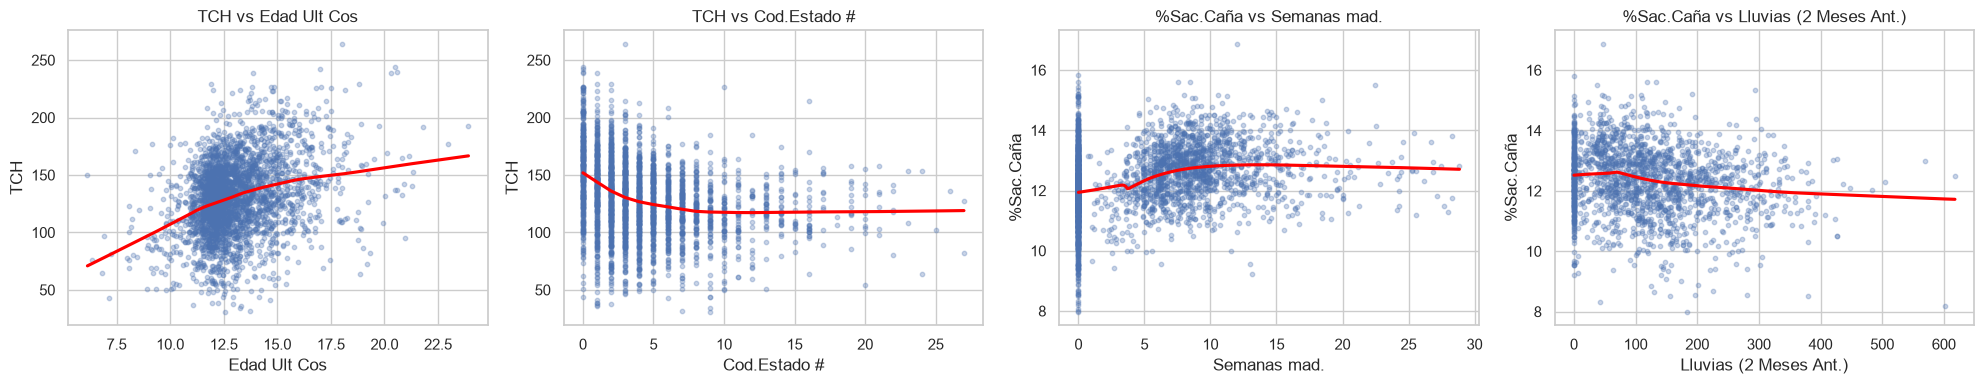
\includegraphics[width=\textwidth]{figuras/dispersion.png}
\caption{Relación del TCH y del \%Sac.Caña con sus principales predictores (muestra de $3\,000$ suertes). La línea roja es una tendencia LOWESS.}
\label{fig:dispersion}
\end{figure*}

\subsection{Regresión}
\textbf{Modelo de referencia.} La regresión lineal múltiple es significativa en conjunto (prueba $F$, $p<0{,}001$), aunque explica solo cerca del $30\,\%$ de la variabilidad ($R^2$ ajustado de $0{,}296$ para TCH y $0{,}294$ para \%Sac.Caña). Con las variables numéricas estandarizadas, los coeficientes indican el cambio del objetivo por cada desviación estándar del predictor. Para el TCH, el mayor efecto corresponde a la edad de cosecha ($+8{,}5$~t/ha), seguida del número de corte ($-5{,}0$~t/ha), la ausencia de registro de lluvia ($-3{,}5$~t/ha), la distancia al ingenio ($-3{,}4$~t/ha) y el volumen de riego ($+2{,}6$~t/ha), todos con $p<0{,}001$; además, $52$ de las $67$ categorías de variedad, suelo y zona resultaron significativas. Para la sacarosa, los efectos dominantes son los de maduración y clima: lluvia en los dos meses previos ($-0{,}26$ puntos), semanas de maduración ($+0{,}23$), dosis de madurante ($+0{,}15$) y mes de corte ($+0{,}09$), mientras que la edad de cosecha y el número de corte no son significativos ($p>0{,}05$). Estos signos son coherentes con la agronomía del cultivo~\cite{cenicana,actaagronomica}.

En cuanto a los supuestos, los residuos se distribuyen alrededor de cero sin patrones marcados, con una distribución simétrica pero de colas pesadas. La prueba de Breusch-Pagan detecta heterocedasticidad en ambos modelos ($p<0{,}001$), por lo que los errores estándar, y con ellos los valores $p$, deben interpretarse con cautela.

\textbf{Modelos avanzados.} La Tabla~\ref{tab:regresion} muestra que los modelos de árboles superan ampliamente a la regresión lineal. XGBoost obtuvo el mejor desempeño: para el TCH elevó el $R^2$ de $0{,}30$ a $0{,}53$ y redujo el RMSE de $27{,}1$ a $22{,}2$~t/ha ($18\,\%$ menos error); para la sacarosa elevó el $R^2$ de $0{,}28$ a $0{,}45$, prácticamente empatado con Random Forest. El RMSE de validación cruzada es similar al de prueba en todos los modelos, lo que descarta sobreajuste. Esta mejora confirma lo observado en el análisis exploratorio: las relaciones son no lineales (mesetas en la edad y en la maduración) y existen interacciones entre variedad, suelo y ubicación que un modelo lineal no captura~\cite{revision2025a,revision2025b}.

\begin{table}[!t]
\caption{Desempeño de los modelos de regresión (conjunto de prueba)}
\label{tab:regresion}
\centering
\begin{tabular}{llccc}
\toprule
Objetivo & Modelo & $R^2$ & RMSE & MAE \\
\midrule
TCH (t/ha) & Regresión lineal & $0{,}296$ & $27{,}05$ & $20{,}82$ \\
           & Random Forest    & $0{,}471$ & $23{,}44$ & $17{,}50$ \\
           & \textbf{XGBoost} & $\mathbf{0{,}526}$ & $\mathbf{22{,}20}$ & $\mathbf{16{,}49}$ \\
\midrule
\%Sac.Caña & Regresión lineal & $0{,}283$ & $0{,}947$ & $0{,}742$ \\
           & Random Forest    & $0{,}453$ & $0{,}827$ & $0{,}639$ \\
           & \textbf{XGBoost} & $\mathbf{0{,}454}$ & $\mathbf{0{,}826}$ & $\mathbf{0{,}637}$ \\
\bottomrule
\end{tabular}
\end{table}

La importancia por permutación de XGBoost (Fig.~\ref{fig:importancia}) mide cuánto empeora el RMSE al desordenar cada variable. Para el TCH, la variable más influyente es la distancia al ingenio, que es prácticamente constante dentro de cada hacienda y actúa como un indicador de su ubicación y sus prácticas de manejo; le siguen la edad de cosecha, la variedad, la edad de la plantación y el suelo, factores señalados en la introducción~\cite{cenicana}. Para la sacarosa dominan las semanas de maduración, el mes de corte (estacionalidad), la variedad y la lluvia previa a la cosecha, en línea con la importancia de la maduración y del clima en la acumulación de azúcar~\cite{cenicana}. En ambos objetivos, los valores predichos tienden a concentrarse cerca del promedio: el modelo sobrestima los rendimientos bajos y subestima los altos.

\begin{figure*}[!t]
\centering
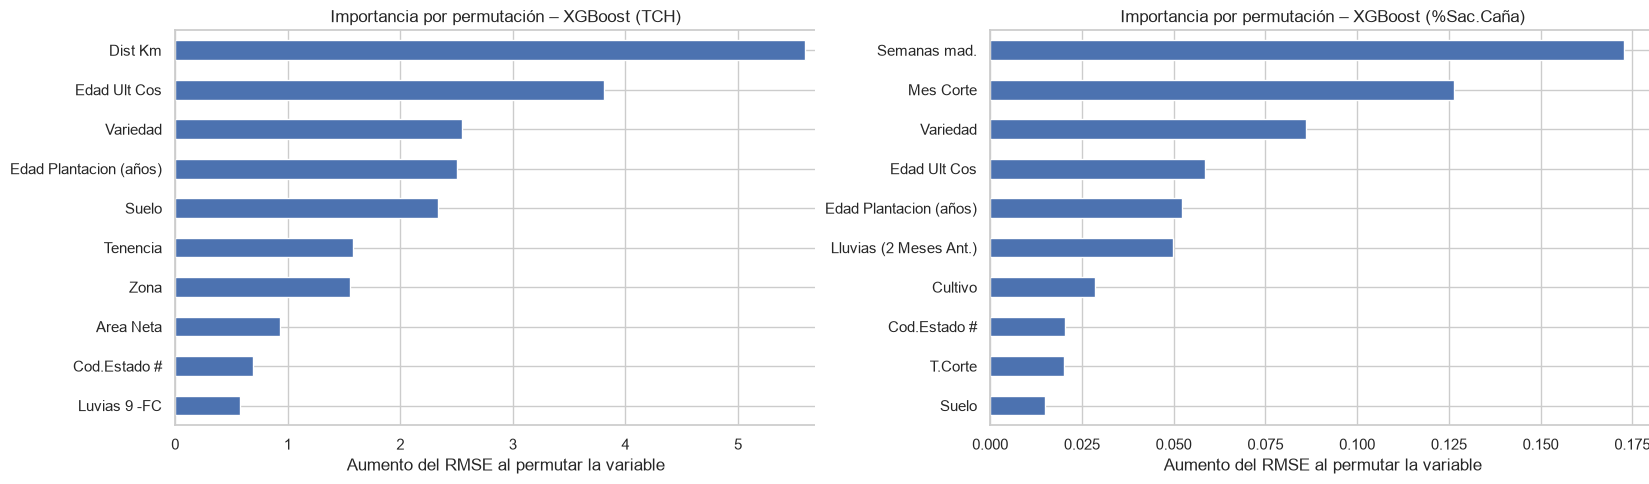
\includegraphics[width=\textwidth]{figuras/importancia_regresion.png}
\caption{Importancia por permutación de las diez variables más influyentes en los modelos XGBoost de TCH (izquierda) y \%Sac.Caña (derecha).}
\label{fig:importancia}
\end{figure*}

El desempeño moderado ($R^2\approx0{,}5$) se explica por la información ausente en los datos más que por los modelos: el $37\,\%$ de las suertes no tiene lluvias registradas, y las variables de clima, fertilización y plagas se descartaron por superar el $50\,\%$ de faltantes. Un $R^2$ cercano a $1$ solo se habría obtenido incluyendo variables con fuga de información, como \textit{TCHM} o \textit{TonUltCorte}, lo que produciría un modelo inútil en la práctica.

\subsection{Clasificación}
\textbf{Modelos de referencia.} En la regresión logística multinomial, la validación cruzada eligió la regularización L1 para ambos objetivos. Para el nivel de TCH, un mayor número de cortes reduce la probabilidad de la clase Alta (coeficiente $-0{,}44$), mientras que la edad y la dosis de madurante la favorecen. Para el nivel de sacarosa, la lluvia empuja hacia la clase Baja ($+0{,}52$) y las semanas de maduración hacia la Alta ($+0{,}41$); L1 eliminó por completo la edad y la dosis de madurante, cuya información queda contenida en las semanas de maduración. La clase Media casi no conserva coeficientes distintos de cero, lo que indica que no tiene un perfil propio y se define por exclusión de las otras dos.

En KNN, el $k$ óptimo para la sacarosa fue $39$: promediar muchos vecinos suaviza el ruido, señal de una relación débil pero consistente. Para el TCH, en cambio, el óptimo fue $k=1$. Este resultado se explica porque el $62\,\%$ de los registros de IPSA comparte hacienda y periodo con otros lotes (mismas lluvias y mismo mes), de modo que el modelo identifica un ``lote hermano'' de la misma hacienda en lugar de aprender una relación agronómica. Es una limitación de la validación aleatoria que una validación agrupada por hacienda corregiría.

\textbf{Comparación.} Todos los modelos superan el $33\,\%$ de exactitud que obtendría el azar con clases balanceadas (Tabla~\ref{tab:clasificacion}). Los mejores fueron Random Forest para el nivel de TCH ($49{,}5\,\%$ de exactitud y Kappa de $0{,}24$) y XGBoost para el nivel de sacarosa ($52{,}3\,\%$ y Kappa de $0{,}28$), con mejoras de $11$ y $8$ puntos frente a la regresión logística. Un Kappa entre $0{,}2$ y $0{,}3$ indica un acuerdo aceptable por encima del azar.

\begin{table}[!t]
\caption{Desempeño de los modelos de clasificación (conjunto de prueba; azar = 33\,\%)}
\label{tab:clasificacion}
\centering
\begin{tabular}{llccc}
\toprule
Objetivo & Modelo & Accuracy & F1 & Kappa \\
\midrule
TCH      & Reg. logística (L1) & $0{,}388$ & $0{,}374$ & $0{,}078$ \\
         & KNN ($k=1$)         & $0{,}450$ & $0{,}450$ & $0{,}175$ \\
         & \textbf{Random Forest} & $\mathbf{0{,}495}$ & $\mathbf{0{,}491}$ & $\mathbf{0{,}242}$ \\
         & XGBoost             & $0{,}441$ & $0{,}438$ & $0{,}160$ \\
\midrule
Sacarosa & Reg. logística (L1) & $0{,}443$ & $0{,}420$ & $0{,}160$ \\
         & KNN ($k=39$)        & $0{,}445$ & $0{,}433$ & $0{,}165$ \\
         & Random Forest       & $0{,}502$ & $0{,}475$ & $0{,}250$ \\
         & \textbf{XGBoost}    & $\mathbf{0{,}523}$ & $\mathbf{0{,}516}$ & $\mathbf{0{,}283}$ \\
\bottomrule
\end{tabular}
\end{table}

Las matrices de confusión (Fig.~\ref{fig:confusion}) muestran que la clase Media es la más difícil de identificar ($55$ de $141$ aciertos en TCH y $49$ de $142$ en sacarosa), ya que corresponde a una franja angosta ($20$~t/ha y $0{,}7$ puntos de sacarosa). Las clases extremas se reconocen mejor, y en la sacarosa la confusión grave entre Baja y Alta es poco frecuente ($19$ y $20$ casos). Según la importancia por permutación, el nivel de TCH depende principalmente del número de cortes, la infestación por diatrea y el mes, y el nivel de sacarosa del mes, las lluvias y las semanas de maduración, el mismo patrón obtenido en la regresión. El desempeño moderado se explica por el menor tamaño de IPSA, la ausencia de variedad y suelo como predictores (todo el dataset es de la variedad CC01-1940) y el $31\,\%$ de lluvias sin registro.

\begin{figure}[!t]
\centering
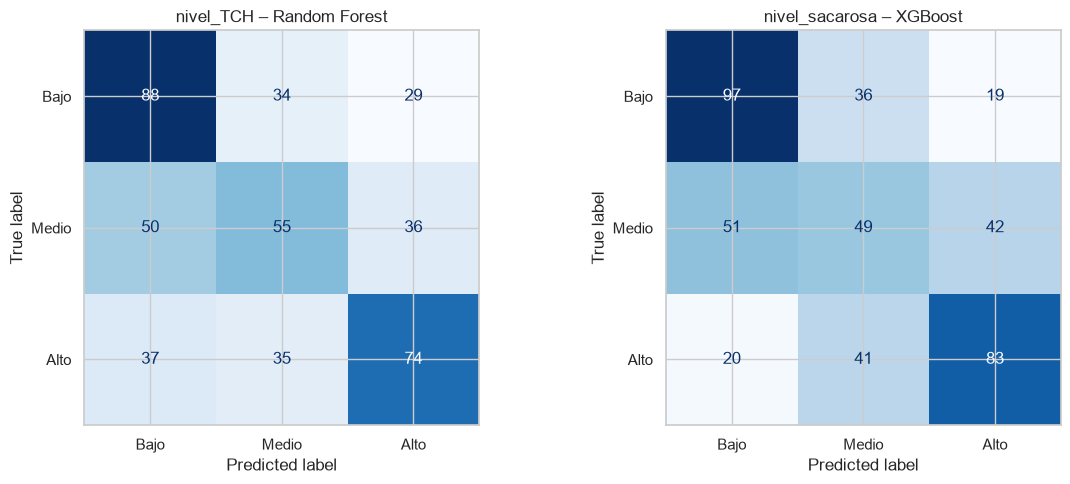
\includegraphics[width=\columnwidth]{figuras/matrices_confusion.png}
\caption{Matrices de confusión de los mejores modelos: Random Forest para el nivel de TCH y XGBoost para el nivel de sacarosa.}
\label{fig:confusion}
\end{figure}

% =====================================================================
\section{Conclusiones y Trabajo Futuro}
% =====================================================================
Los modelos de ensamble basados en árboles superaron a los modelos de referencia en las cuatro tareas: XGBoost redujo el error de predicción del TCH en un $18\,\%$ y el de la sacarosa en un $13\,\%$ frente a la regresión lineal, y en clasificación los mejores modelos superaron a la regresión logística en $8$ a $11$ puntos de exactitud. Esto confirma que las relaciones entre el manejo agronómico, el clima y el rendimiento son no lineales. Las variables más influyentes coinciden con el conocimiento agronómico: la edad de cosecha, el número de corte, la variedad y la ubicación determinan las toneladas, mientras que la sacarosa depende de la maduración, de la lluvia previa al corte y de la época de cosecha.

Para el Ingenio Providencia, estos modelos pueden apoyar la planificación de la cosecha, al anticipar qué suertes tendrán un rendimiento bajo, y la programación de la maduración, al evidenciar el efecto de las semanas de maduración y de la lluvia sobre la sacarosa. El análisis del cultivo orgánico muestra, además, que las prácticas sostenibles sin madurantes químicos tienen un costo en calidad que el ingenio puede cuantificar y compensar con otras estrategias.

\textbf{Trabajo futuro.} La principal línea de mejora es completar la información disponible: integrar índices de vegetación obtenidos de imágenes satelitales (por ejemplo, NDVI), datos completos de estaciones climáticas y registros reales de fertilización y plagas. También se propone evaluar los modelos con validación agrupada por hacienda (\textit{GroupKFold}) para medir su capacidad de generalizar a fincas no vistas, y avanzar hacia un sistema de monitoreo en tiempo real que actualice las predicciones con sensores de campo durante el ciclo del cultivo y reentrene los modelos al final de cada zafra.

\textbf{Limitaciones.} Los modelos identifican asociaciones, no relaciones causales, por lo que no deben usarse por sí solos para decidir prácticas de manejo. El dataset de clasificación corresponde a una sola variedad, de modo que sus resultados no se generalizan a otras variedades ni a otros ingenios. Desde el punto de vista ético, las predicciones no deberían emplearse para evaluar o penalizar a cultivadores proveedores sin considerar factores fuera de su control, como el clima, y su uso debe ser transparente y complementar el criterio de los expertos agronómicos.

% =====================================================================
%   REFERENCIAS (formato IEEE)
% =====================================================================
\begin{thebibliography}{00}
\bibitem{asocana} Asocaña, ``Informe Anual 2024--2025: aspectos generales del sector agroindustrial de la caña,'' Asociación de Cultivadores de Caña de Azúcar de Colombia, Cali, Colombia, 2025. [En línea]. Disponible: \url{https://www.asocana.org/modules/documentos/17797.aspx}
\bibitem{cenicana} Cenicaña, \textit{Informe Anual 2023}. Cali, Colombia: Centro de Investigación de la Caña de Azúcar de Colombia, 2024. [En línea]. Disponible: \url{https://www.cenicana.org/en/annual-report/}
\bibitem{actaagronomica} C. A. Viveros Valens, D. Baena García, F. Salazar Villareal, L. O. López y J. I. Victoria K., ``Características de la caña de azúcar asociadas con toneladas de caña por hectárea y sacarosa (\% caña),'' \textit{Acta Agronómica}, vol. 64, no. 3, pp. 268--272, 2015, doi: 10.15446/acag.v64n3.44494.
\bibitem{providencia} Ingenio Providencia S.A., ``Informe de Sostenibilidad 2024,'' Valle del Cauca, Colombia, 2025.
\bibitem{revision2025a} S. Salgado-Velázquez, H. Becerril Hernández, J. A. Rincón-Ramírez, L. Aceves-Navarro y S. Córdova-Sánchez, ``Remote sensing and machine learning techniques used to predict sugarcane (\textit{Saccharum} spp.) yield,'' \textit{Agro Productividad}, vol. 18, no. 9, pp. 229--237, 2025, doi: 10.32854/dp4qtd40.
\bibitem{revision2025b} S. M. Shawon \textit{et al.}, ``Crop yield prediction using machine learning: An extensive and systematic literature review,'' \textit{Smart Agricultural Technology}, vol. 10, art. no. 100718, 2025, doi: 10.1016/j.atech.2024.100718.
\end{thebibliography}

\end{document}